\begin{savequote}[8cm]
  ``He who controls the past controls the future.''
  \qauthor{George Orwell, 1984}
\end{savequote}
\makeatletter
\chapter{Literature Review}

\section{Introduction}

\section{3D Reconstruction and Simultaneous Localization and Mapping}
\subsection{Introduction}
hi there
\subsection{Monocular Camera Feature Based Systems}
Monocular Feature based SLAM systems use feature matches to estimate camera pose and location changes across frames \cite{Davison02Simultaneous}. Variations of this method use different features including: corners and lines \cite{Jeong06Visual}, image patches \cite{Silveira08Efficient} and exemplar feature matching \cite{Chekhlov07Robust}. SIFT features are used most often in SLAM \cite{Jensfelt06Framework,Pollefeys08Detailed,Beall11Bundle,Eudes10Fast}, in addition FAST features have been explored \cite{Kundu10Realtime,Leelasawassuk133d,Konolige10View,Konolige08Frameslam}. Beall et al \cite{Beall11Bundle} made use of both SIFT and SURF features in their underwater SLAM system. Real-time monocular SLAM systems based on this approach have also been proposed \cite{Chekhlov07Robust,Pollefeys08Detailed}. RANSAC is often used in monocular SLAM \cite{Eudes10Fast,Kundu10Realtime,Konolige10View,Konolige08Frameslam,Pradeep13Monofusion} to remove outliers which cause incorrect camera parameter estimates. Bundle adjustment is also used as an additional step to refine camera parameter estimation \cite{Eudes10Fast}. 
\subsection{Stereo Camera Feature Based Systems}
Stereo based SLAM systems also use features to estimate camera parameters. However, stereo based systems are capable of generating dense depth data more easily using stereo algorithms. Miro et al \cite{Miro06Towards} proposed a stereo based method which uses SIFT and the extended Kalman filter. The method by Van Gool et al \cite{Pollefeys04Visual} works with un-calibrated stereo pairs. It uses Harris corner features and a multi-view stereo algorithm. Sim et al \cite{Sim05Vision} and Gil et al \cite{Gil06Improving} both presented stereo based SLAM systems which use SIFT.


\subsection{Kinect Fusion}

Newcombe et al \cite{Newcombe11Kinectfusion} proposed an accurate, real-time dense 3d reconstruction algorithm which works well on complex indoor environments. This algorithm computes relationships between depth map frames generated using the Microsoft Kinect \cite{Zhang12Microsoft} sensor. By aligning depth maps this method is capable of tracking both camera pose and location as well as generating dense 3d reconstructions. Only depth data is used in alignment computations thus, consequently because the Kinect is a structured light based depth sensor Kinect Fusion works under any lighting condition, including complete darkness. Since they use the Kinect and GPU (both considered commodity hardware these days) the technique may be considered inexpensive. \\

The method works by computing camera pose, transforming depth data by a computed pose (frame-by-frame) and fusing this data into a global surface volume. It uses a coarse to fine grain iterative closest point (ICP) algorithm to compute camera pose. During the ICP phase, the target points come from the entire globally matched previous frames. Therefore this method is considered global rather than frame-to-frame based. Such a method has direct advantages over frame-by-frame feature matching, since all data is used to compute pose. The downside, is that this method fails to find global solutions due to the nature of ICP. This may occur when some frames must be skipped due to motion blur, or the camera passing over surfaces which do not reflect infra-red light. \\

\begin{figure}[!h]
\centering
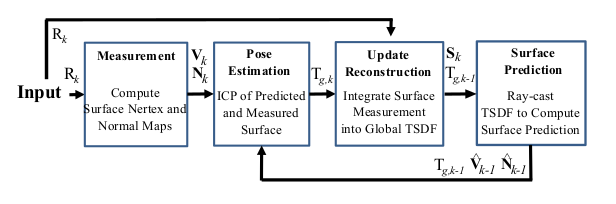
\includegraphics[width=12cm]{images/ch1/Newcombe11KinectFusion1}
\caption{Kinect Fusion Algorithm Pipeline \cite{Newcombe11Kinectfusion}}
\label{KFusionPipeline}
\end{figure}

Kinect Fusion has four main steps as illustrated in figure \ref{KFusionPipeline}. The first step named measurement, performs pre-processing on the depth data as well as generation of additional information for use by Kinect Fusion. Each depth map frame is first passed through a bilateral filter. From this, a dense vertex map (map of 3D points projected using a known projection matrix associated with the Kinect) is generated, as well as a normal map. For both the vertex and normal maps, a 3 level image pyramid is constructed. This makes the coarse to fine grain ICP technique possible. \\

Next, dense coarse to fine grain ICP is used to compute pose between the fused frames and the current frame. The authors exploit the fact that the transformation between frames is small because camera motion is slow when computing against every frame. With coarse-to-fine grain ICP they use the point-plane metric for pose optimization \cite{Rusinkiewicz02Real}. The ICP based pose estimation computes pose given both a predicted and measured depth map. \\

After estimating camera pose relating to the globally fused model, each frame must be integrated into that model. The Kinect Fusion algorithm uses a truncated signed distance function (TSDF) representation. This is a signed distance function volume where the distances for each voxel are capped by some value. The TSDF uses a volume resolution of $512\times 512\times 512$. They use the TSDF, rather than relying on a linear but accurate discrete SDF transform \cite{Rasch09Remarks} because of the computational complexity of calculating the discrete SDF of large scale volumes. \\

As mentioned, Kinect fusion uses pose prediction and fuses each depth map into the TSDF representation. In this way, they align and fuse each depth map to the global 3d reconstruction. In this way, a global loop closure method is not required. This may have a negative side effect by which some frames which have larger resolutions may be heavily quantized in order to fuse with the SDF, especially very thin surfaces/objects. These features may also be advantageous for ICP in estimating pose. 



\subsection{3D Reconstruction by Optimizing directly in the SDF}

In 2013, Bylow et al \cite{Bylow13Real} presented a novel method which reconstructs static indoor environments in real time using RGB-D data captured using the Asus Xtion Pro Live sensor. Their system is able to generate accurate 3D RGB coloured models of the environment in real-time by optimizing for 6 degrees of freedom in terms of accurate projection of new depth map frames into an existing global signed distance function model of the scene. Their method uses several Gauss Newton optimization with a signed distance function representation, these techniques are represented and processed using a laptop with an NVIDIA GPU. Unlike Kinect Fusion \cite{Newcombe11Kinectfusion}, this method optimizes directly in the signed distance representation, in which camera pose is computed by finding a rotation and translation (6-DoF) which minimizes the error of projecting depth images into the SDF. Compared with the ICP based method used by Kinect Fusion, this technique is shown to be more robust and accurate. It compares favourably to bundle adjustment but is much faster for small to mid sized scenes. Results are generated using the TUM RGB-D benchmark and SDF volume sizes $256^3$ and $512^3$ are used in evaluations. The authors note the algorithm may be able to handle large scale scenes if used in conjunction with other techniques \cite{Kaess11Isam2,Kummerle11G}. \\

This technique is efficient because the error to minimize can be checked using several look-ups since the SDF itself contains the distances from each voxel to the global model's actual surface. Because of this, the algorithm is classified as working within global space rather than frame-by-frame. Using the SDF to lookup depth map projection error, the camera pose is iteratively estimated and then the depth map is integrated into the SDF and colour information is stored in another volume. The pose estimation procedure begins by storing the first frame as a volumetric signed distance function. Then for each new depth frame, camera pose is computed, and based on this pose the frame is projected into the scene. Using a lie algebra based 6-DoF model \cite{Ma12Invitation} envisioned as a vector in $R^6$ representing camera pose, the error for a given pose may be computed as the squared error of the depth map transformed by the pose and projected into the signed distance function. Due to noise or missing data within the depth frame, this error may never be reduced completely, instead the best pose is iteratively computed using this model and the Gauss Newton non-linear optimization algorithm. \\

The SDF representation uses two volumes as in \cite{Curless96Volumetric}, one volume stores the average distances, the other stores the cumulative weights for each voxel. Bylow et al use these weights to handle occlusion and sensor uncertainty. When integrating a point into the SDF, tri-linear interpolation is used between eight neighbours to handle point coordinated made up of floating point numbers. During integration, each voxel is projected onto the image plane rather than ray case from the center of projection as in \cite{Newcombe11Kinectfusion}. This ensures that each voxel is visited once when updating the SDF, whereas in the ray casting approach, this may not necessarily be the case. \\

In computing the SDF for a given depth map, the exhaustive marching cubes algorithm is too slow, even the fast marching algorithm \cite{Baerentzen01Implementation} is not suited for real time discrete SDF generation. Instead, the SDF is approximated with either the point to point distance or point to plane distance functions. For final visualization, marching cubes is used \cite{Lorensen87Marching} on the final SDF. Colour is computed from the colour volume using a technique found used by Whelan et al \cite{Whelan13Robust}. Since the method by Bylow et al is based on optimizing the projection error using the SDF and only uses locations in its pose estimation procedure, it is independent to illumination. Given this, it will also fail in cases where only co-planar surfaces are visible, they mention that using colour information during tracking \cite{Kerl13Robust} may mitigate these concerns.


but kinect fusion generates synthetic depth images which are aligned to the current depth image using icp


\subsection{Sturm}

approach to SLAM for RGB-D cameras (eg. kinect)
computes dense 3d environment + computes camera pose
evaluated at different illuminations + camera speed conditions
evaluates 3 different features SIFT, ORB and SURF
system can deal with difficult data in common indoor scenarios and is fast enough for online operation
1st : extract features from color image data, match with previous frames
this gives point-wise 3d matches
then - RANSAC may be used to compute the transform between 3d frames
because frame-by-frame is not globally consistent
optimize the pose graph in a fourth step using the g2o solver [11] optimizes non-linear error functions
uses octomap [33] to generate a volumetric representation of the environment
uses datasets [29]
handles up to 50 deg per sec / ,43 meters per sec
voxelizes using octomap, uses 3d occupancy grid for output

SLAM used in robotics [30,22,10,6,15,9,23]
modern systems use ICP [2, 26, 27]
vslam [5, 16, 28, 14, 21] => get sparse keypoints,  
these simplify data association
sift[20, surf[1], orb[25]], sift gpu[32]


in monocular setting, the scale of the map cannot be  determined

stereo slam [17, 24] -> does not suffer from this
only accurate for textured surfaces, non-textured surfaces cannot be estimated with depth

Fioraio [7] presented a system which uses bunfle adjustment to align rgb-d data

henry [12] is similar to this work

uses sparse keypoint matches between color images as initialization to icp

icp often not necessary and expensive
icp only used if no keypoint matches found...

henry used sparse bundle adjustment [19], here 3d pose graph using [18] framework is used

henry put resulting into surfel representation, here volumetric voxel representation is used [33], can be used for robot localization, path planning and navigation [13]

figure 2 has a picture

front-end: keypoint det, match, sensor pose from ransac
back-end: optimizes poses with non-linear error function
	computes optimal sensor positions using a graph-based routine -> then the occupancy voxel grid map is computed
	
front-end details: 
uses opencv [3] for detection, description and matching of features SURF, SIFT and ORB [25], for SIFT: GPUSIFT[32]

ORB is based on FAST [25] and BRIEF[4]

ORB computes orientation from FAST corners and uses for descriptor extraction -> so it is more robust to viewpoint changes (faster than both sift and surf)

sets the hessian threshold to keep number of keypoints constant, too few keypoints and there may be not enough matches, too many and there may be too many false positives

then the transformation of camera pose can be computed from these correspondences [31]


because of synchronization at the shutters of infrared and color camera and due to interpolation at depth jumps
plus because features often lie at object borders, 3d features positions are prone to be at a wrong depth making robust estimation of transformations highly non-trivial

RANSAC known to cope with noise data [8]
points considered inliers if after transformation their distance is < 3cm

then, the inliers are used to compute a finer representation, these steps are repeated where most inliers are kept

















[BG Bylow]

bundle adjustment using features over many views with [13 \cite{Klein07Parallel} , 2 \cite{Agarwal09Building}] with sparse 3d models generated

algorithms to compute dense depth maps from image data [10 \cite{Hirschmuller05Accurate} , 21 \cite{Stuhmer10Real}]

newcombe [18 \cite{Newcombe11Kinectfusion} ] -> impressive results using sdfs to represent reconstruction, and icp for camera tracking

whelan [24 \cite{Whelan13Robust}] estended with rolling reconstruction volume and color fusion, evaluated alternative methods for visual odometry estimation

pure visual odometry induces significant drift, so matching with global model is their preference

novel method of estimating camera motion directly based on the SDF, key insight : sdf encodes distance to surface

do not need downsampling in case of icp to achieve real time performance

comparable to the feature based rgb-d slam [8 \cite{Endres12Evaluation}]

icp[4 \cite{Besl92Method}]

graph slam use motion estimates as input to construct and optimiza a pose graph[15 \cite{Kummerle11G}] these methods render a joint map only after pose graph optimization

this map is generally not used for further optimization

the resulting maps are often represented as occupancy grid maps or octrees [25 \cite{Wurm10Octomap}]

henry [9 \cite{Henry10Rgb}], applied graph slam to rgb-d data, using visual features + icp combo [8] also did a similar system, on benchmark [22 \cite{Sturm12Benchmark}]

[18 \cite{Newcombe11Kinectfusion} dense 3d recon possible with realtime, 

sdf[7 \cite{Curless96Volumetric}]

KF: for each image:
it renders a point cloud from the sdf at the previous pose using ray tracing and aligns this with the depth image


point correspondences are found using projective data association [5 \cite{Blais95Registering}] and the point to plane distance

Kin-Fu open source implementation available in the PCL library

(icp only minimizes error on point clouds, some other approaches minimize photometric error [20 \cite{Steinbrucker11Real}, 12 \cite{Kerl13Robust}]

or combinations of both [23 \cite{Tykkala11Direct}]) -> these did not perform 3d reconstruction

whelan integrated these methods with kinect fusion [24 \cite{Whelan13Robust}]

Canelhas [6 \cite{Canelhas12Scene}] did masters thesis an approach for camera tracking, similar to this
his focus concentrates on object detection and recognition in an sdf and no thorough evaluation was performed

Kubacki [14 \cite{Kubacki12Registration}] showed how an sdf can be used to estimate camera pose, only on synthetic data without a comparative evaluation

[19 \cite{Ren12Unified}] demonstrated sdf based object tracking, based on known models

presented by Bylow: direct approach to camera tracking on sdfs


stable enough for use with quadcopter























[Background from KF]

area promises new augmented reality and mixed reality applications

SFM and MVS (multi view stereo) has given good results : camera tracking  and sparse reconstructions [10] \cite{Fitzgibbon98Automatic}, \cite{Seitz06Comparison} [24] 

SLAM has focused on real time markerless tracking and live scene reconstruction based on a single sensor RGB eg. MonoSLAM[8] \cite{Davison03Real} which is less accurate than PTAM [17] \cite{Klein07Parallel}  but these only produce sparse reconstructions

some methods have grown to combine PTAM's camera tracking ability with MVS-style reconstructions [19/26] (\cite{Newcombe10Live}/\cite{Stuhmer10Real})

recently: iterative image alignment has been used to replace features in tracking [20] \cite{Newcombe11Dtam}

this scene is promising: but monocular based dense 3D reconstruction is difficult and requires suitable camera motion and scene illumination

camera technologies have also been evolving: enter the world of new depth cameras or rgb-d cameras,
these have become available to consumers and may soon be found in mobile technologies \cite{Zhang12Microsoft}

first real-time rgb-d depth sensor : with this system users can wave around the device to generate smooth, continuously updating, fully reconstructed data: using only depth, 6dof are tracked

works in full darkness : mitigating issues for passive cameras: [17 \cite{Klein07Parallel} /19 \cite{Newcombe10Live} /26 \cite{Stuhmer10Real}] and other rgb systems [14 \cite{Henry10Rgb}]

[XYZ]

kw : dense volumetric reconstruction

GPGPU kw: is one of their design keys, their system can perform in real time at above these frame rates

they perform qualitative analysis

Kinect: incorporates a structured light based depth sensor, uses an on board ASIC generating an 11-bit 640x480 depth map at 30hz

depth images often contain holes : this is an issue (caused by no structured light could be read on the surface, certain materials, which do not reflect infra-red light (very thin structures or surfaces at incendence angles

when moving fast, the device can also experience motion blur, this leads to missing data

then they do  reviews on:
	slam, dense tracking, surface representations, previous work with joint tracking and modelling using depth sensors

[Background]

early sfm algorithms: either accumulated drift (computing motion) [2 \cite{Beardsley97Sequential} ] or performed loop-closure using off-line optimization 

The first monocular slam system [8 \cite{Davison03Real} ] was capable of producing globally consistent maps in real time with hand-held camera used probabilistic filtering of camera and scene feature estimates

limited to in-door office environments because it requires large state vectors which grow with scene size
sparse feature maps lead to poor accuracy

then systems which split tracking and mapping (global optimization) -> approach by PTAM system [17 \cite{Klein07Parallel}]
: real time mono slam in work spaces -> basically it is just bundle adjustment (which is the least squares solution to camera and feature optimization (theirs chooses features dynamically over the frame range)

their tracking system runs in parallel at frame-rate speeds, and performs robust n-point pose estimation with feature matching

compared to filters much more features can be packed into the map[25 \cite{Strasdat10Real} ]

PTAM = realtime results as accurate as off-line ones

PTAM produces sparse maps - not like our project

some algorithms can use PTAM tracking in conjunction with dense reconstruction computing module based on multi-view stereo

[19 \cite{Newcombe10Live}] uses dense optical flow with PTAM like tracking for dense recon

this relies on camera poses coming from PTAM

[26 \cite{Stuhmer10Real}] do the same with near real time depth map calculation

DENSE TRACKING AND MAPPING by Scan Alignment

dense sensor based 3d reconstruction research has continued using lasers and depth sensors

typically : minimize distance measures between all data rather than feature extraction and matching

6dof camera alignment and 3d surface reconstruction techniques developed in the graphics domain, here ICP is the most important
ICP @ [3 \cite{Besl92Method} ]

ICP is a non-linear optimization problem where approximations are found using the closest points currently for each
set

distance metrics have been researched using the point-plane metric [5 \cite{Chen92Object}]

[\cite{Chen92Object} 5] improves convergence rates, used for surface reconstructions which have normal data

computing closest points using ICP is expensive, there is projective data association algorithm [4 \cite{Blais95Registering}]

can be used for data in projective form (2d image where each image is a 3d point)

can reduce icp set to possible set of points or with a coarse to fine scheme

SLAM may use ICP to estimate camera changes

Dense 3D scene representations:

occupancy mapping : use a grid to store data

[9 \cite{Elfes87Sensor}] uses a Bayesian probability of occupancy to measure whether should be added to the grid

also can used signed distance functions [9 \cite{Elfes87Sensor}] (SDF), it can be used to fuse partial depth scans, whilst mitigating
issues relating mesh-based reconstruction algorithms

SDF represents : surface interfaces as 0, positive values that increase with distance from the nearest surface
and occupied space using a negative value

more robust to noise version of SDF -> [30 \cite{Zach07Globally} ]

SDF can be visualized by first converting to mesh and rendering ( use marching cubes [18 \cite{Cubes87High}]) or it can be directly ray cast [21 \cite{Parker98Interactive}]

[23 \cite{Rusinkiewicz02Real}] used frame-by-frame ICP with occupancy grid, users can scan in small objects by rotating the objects with their hand
works @ 10hz, issue: does not do global optimization, cannot do large scenes . final models are optimized using [7 \cite{Curless96Volumetric}]
sdf fusion in real time may be possible

sdf can be used for globally satisfying reconstruction

small scale reconstructions:
	[28 \cite{Weise09Hand}] -> produces high quality scans using a fixed ToF sensor
	[6 \cite{Cui103d} ] demonstrate a moving handheld ToF scanner

Octomap [29 \cite{Wurm10Octomap}] -> 3d reconstruction using occupancy grid style 

[14 \cite{Henry10Rgb}] uses rgb-d with kinect by frame by frame icp : feature matching is used with graph optimization for loop closure and global consistency -> global fusion presents better performance








































\ref{Newcombe11Kinectfusion}

\subsection{RGB-D Sensor Feature Based Systems}
RGB-D SLAM systems use both depth and image data and are capable of generating dense 3D reconstructions. Many of these methods rely on feature matching techniques \cite{Engelhard11Real,Henry10Rgb,Endres12Evaluation}. RANSAC is often used to filter outliers for the estimation of camera parameters\cite{Engelhard11Real,Henry10Rgb,Endres12Evaluation}. Another method which has also been used extensively in the area is Iterative Closest Point (ICP) \cite{Engelhard11Real,Henry10Rgb,Bylow13Real,Newcombe11Kinectfusion,Stuckler12Robust,Izadi11Kinectfusion}. ICP iteratively registers point cloud data, and is used to refine camera parameter estimates. A method named KinectFusion was proposed by Newcombe et al \cite{Newcombe11Kinectfusion} which uses RANSAC and a GPU implementation of IPC. Whelan et al \cite{Whelan12Kintinuous} extended this method allowing it to map larger areas using Fast Odometry From Vision (FOVIS) over ICP. Bylow et al \cite{Bylow13Real} improved the ICP approach by registering data using a signed distance function.
\subsection{Non-Feature Based Methods}
Several RGB-D SLAM systems are also non-feature based \cite{Weikersdorfer14Event,Izadi11Kinectfusion,Kerl13Dense}. Weikersdorfer et al \cite{Weikersdorfer14Event} presented a novel sensor system named D-eDVS along with an event based SLAM algorithm. The D-eDVS sensor combines depth and event driven contrast detection. Rather than using features, it uses all detected data for registration. Kerl et al \cite{Kerl13Dense} proposed a dense RGB-D SLAM system which uses a probabilistic camera parameter estimation procedure. It uses the entire image rather than features to perform SLAM.
\subsection{Summary}
As is evident from the current literature, SLAM typically relies on feature matching and RANSAC. However, these approaches fail when there are too few features, when feature confusion occurs or, when features are non-stationary due to object motion. As the extent of random feature displacement becomes more global the effectiveness of these approaches diminishes. Feature matching also dominates in image registration. However, Fourier based methods have been shown to work well under larger rotations and scales \cite{Gonzalez11Improving} whilst being closed form, insensitive to object motion and scaling naturally to GPU implementations. Accordingly, we propose a novel, closed form Fourier based SLAM method.

Simultaneous localization and mapping (SLAM) has applications in many fields including: robotics, business, architecture and engineering, and science. Its goal is to generate a map (2D birds-eye view, or 3D) of an environment captured by camera and/or other means. In this work we focus on monocular systems, or systems which generate location and mapping data using information generated by a single basic video camera. To this end, current methods rely on the computation of the fundamental and essential matrices. These feature matching techniques fail in cases where features are not stable or where feature confusion occurs. 

It has been shown [1] that using volume registration to compute dense 3D maps is not only independent of feature matching, but it is a closed form solution and is robust to noise and object motion. However, this method requires RGB-D video input provided by special hardware. In this paper we present preliminary results in applying volume registration to generate dense 3D maps from monocular video data. To achieve this, disparity maps are generated between video frames. This data is then used as input for the RGB-D volume registration method.

\section{Feature Matching and RANSAC}

\section{Iterative Closest Point}

\section{Fourier Based Registration}

\section{3D Data Compression Schemes}

\subsection{Model Compression}

The Feature-Oriented Geometric Progressive Lossless Mesh coder (FOLProM) \cite{Peng10Feature} is a state of the art codec which is progressive. It also aims to be an effective low-bitrate codec. It classifies segments of the mesh as being visually salient or not. Salient segments are preserved more during compression compared to non-salient ones. \\

\subsection{Spectral Compression}

Karni and Gotsman \cite{Karni00Spectral} proposed a lossy method which compresses a spectral representation of a mesh. This algorithm generally partitions the mesh and compresses each partition separately since it does not work on large meshes. Encoding a basis function for each partition, coefficients are quantized, truncated and entropy coded. Results show this method outperforms the valence method \cite{touma98triangle} at coarse quantization levels. Bayazit et al. \cite{Bayazit103DMesh} also developed a progressive method based on spectral compression. This method is based on the region adaptive transform in the spectral domain and is advertised as a current state of the art lossy 3D data compression method. \\

\subsection{Wavelet Methods}

A lossy wavelet based compression system was proposed by Khodakovsky et al \cite{Khodakovsky00Progressive}. This technique samples the mesh, and uses the wavelet transform to decorrelate the data. Coefficients are quantized and stored in a structure called a zero tree which increases compression performance. This method is shown to outperform the valence method. Other wavelet approaches \cite{Guskov00Normal,Khodakovsky04Normalmesh} also sample the mesh and use a multi-resolution representation in which the data is described using local normal directions on the mesh surface.

Gu et al \cite{Gu02Geometry} devised a solution for representing 3D models as 2D images which are then compressed using state of the art image compression methods (based on wavelets). To form this representation, the mesh is cut along a network of edge paths, opening the mesh into a topological disk, which is then sampled onto a 2D grid. Each pixel in the image has a corresponding coordinate in the model, with pixel neighbourhoods describing connectivity. Comparisons with the method by Khodakovsky et al reveal the geometry image codec does not have as high compression performance.



\section{Conclusion}

